\documentclass[tikz,border=10pt]{standalone}
\usepackage{pgfplots}
\usetikzlibrary{calc}

\begin{document}
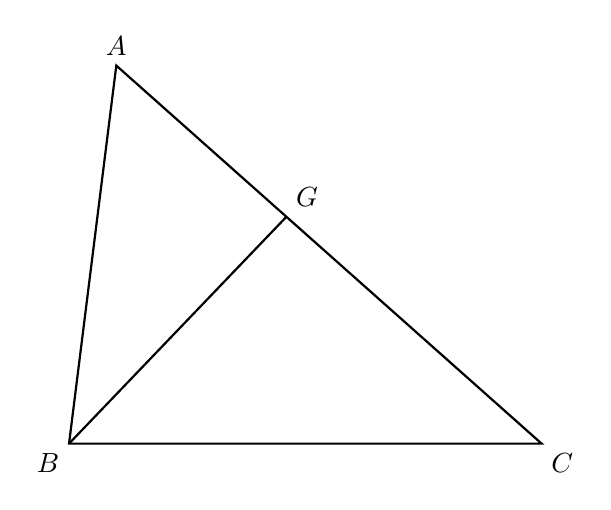
\begin{tikzpicture}[>=stealth, scale=1.2]
    % 1. 定义顶点坐标 (根据图像比例估算)
    \coordinate (B) at (0,0);
    \coordinate (C) at (5,0);
    \coordinate (A) at (0.5,4);
    
    % 2. 计算点 G 的位置 (位于 AC 边上，约位于中间偏上位置)
    % 使用 TikZ 的线性插值语法: (A)!比例!(C)
    \coordinate (G) at ($(A)!0.4!(C)$);

    % 3. 绘制三角形主体和连线
    \draw[thick] (A) -- (B) -- (C) -- cycle; % 绘制三角形 ABC
    \draw[thick] (B) -- (G);               % 绘制连线 BG

    % 4. 标注顶点标签
    % 使用 node 指令放置字母，并通过 [above], [below] 等调整位置
    \node[above] at (A) {$A$};
    \node[below left] at (B) {$B$};
    \node[below right] at (C) {$C$};
    \node[above right] at (G) {$G$};

    % 5. (可选) 如果需要强调点，可以取消下面代码的注释绘制实心圆点
    % \fill (A) circle (1.5pt) (B) circle (1.5pt) (C) circle (1.5pt) (G) circle (1.5pt);

\end{tikzpicture}
\end{document}